\documentclass[11pt]{article}

\usepackage[margin=1in]{geometry}
\usepackage{booktabs}
\usepackage{graphicx}
\usepackage{hyperref}
\usepackage{xcolor}
\usepackage{tikz}
\usetikzlibrary{arrows.meta,positioning}

\title{Learning Predictive World Models from Videos: A Survey on Generative Simulation and Physical Dynamics}
\author{Anonymous}
\date{}

\begin{document}

\maketitle

\begin{abstract}
Predictive world models learned from videos aim to model how visual environments evolve and how future states depend on actions, latent controls, physical interactions, and evaluation criteria. This survey reviews video-based world models as a set of representation and dynamics choices rather than as a list of generative architectures. We compare model families across representation, transition mechanism, conditioning or intervention signal, and evaluation protocol, covering action-conditioned and stochastic video prediction, object-centric physical dynamics, latent and feature-space models for planning and control, diffusion-based and interactive simulators, and benchmarks for physical consistency and world-model validity. The central argument is that visual realism is insufficient: a video world model should also be judged by whether its learned states and dynamics support prediction under interventions, controllable rollout, physical or causal consistency, and downstream decision making. The survey highlights the recurring abstraction-fidelity trade-off between compact states that support efficient control and image-space or token-based models that preserve richer visual detail. It concludes with evaluation principles for future benchmarks that jointly test prediction, control, long-horizon consistency, and physical-law generalization.
\end{abstract}

\section{Introduction}

\paragraph{Section thesis.}
Predictive world models from video have moved from frame prediction toward controllable, structured, generative, and physically evaluated simulators.

\paragraph{Planned subsections.}
\begin{itemize}
  \item Motivation: why video prediction is not yet world modeling.
  \item Conceptual arc: prediction, structure, control, generation, and evaluation.
  \item Scope and evidence policy for this survey.
  \item Contributions and organization.
\end{itemize}

\paragraph{Key claims.}
\begin{itemize}
  \item C001: Action-conditioned video prediction bridges passive prediction and world modeling. Supporting papers: P004 \cite{oh2015_action_conditional_video_prediction_prov}.
  \item C003: Frame quality alone is insufficient for world-model evaluation. Supporting papers: P004 \cite{oh2015_action_conditional_video_prediction_prov}, P009 \cite{janner2019_o2p2_prov}, P012 \cite{alonso2024_diamond_prov}.
  \item C011: Latent world models use compact state dynamics for planning or policy learning. Supporting papers: P001 \cite{hafner2019_planet_prov}, P002 \cite{hafner2020_dreamer_prov}, P003 \cite{ha2018_world_models_prov}.
  \item C021: Visual realism should not be equated with physical correctness. Supporting papers: P037 \cite{bansal2025_videophy_prov}, P012 \cite{alonso2024_diamond_prov}.
  \item C024: Evaluation should go beyond pixel fidelity and reward. Supporting papers: P004 \cite{oh2015_action_conditional_video_prediction_prov}, P012 \cite{alonso2024_diamond_prov}, P013 \cite{bruce2024_genie_prov}, P037 \cite{bansal2025_videophy_prov}.
\end{itemize}

\paragraph{Expected figures and tables.}
\begin{itemize}
  \item Figure 1: Survey landscape from video prediction to physical world models.
\end{itemize}

\paragraph{Missing evidence.}
\begin{itemize}
  \item Broader benchmark support from P033--P040 is pending completed notes. \textbf{[NEEDS SOURCE]}
  \item Diffusion-video lineage notes for P011 and P020 are pending. \textbf{[NEEDS SOURCE]}
  \item Modern latent and interactive model notes for P010, P014--P016, P021, and P022 are pending. \textbf{[NEEDS SOURCE]}
\end{itemize}

\section{Background and Scope}

\subsection{Video Prediction as Predictive Modeling}

Video prediction studies how a model can infer future visual observations from past visual evidence, sometimes with additional conditioning variables such as actions. In its simplest form, the model receives one or more frames and predicts subsequent frames; in action-conditioned settings, the prediction also depends on the intervention an agent will take. Early action-conditioned work made this connection explicit by predicting high-dimensional Atari observations under discrete control inputs, while robot-interaction video prediction used action-conditioned motion transformations to forecast how objects move under manipulation \cite{oh2015_action_conditional_video_prediction_prov,finn2016_physical_interaction_video_prediction_prov}. SV2P illustrates why this task cannot always be reduced to a single deterministic future: latent variables can represent multiple plausible rollouts when the future is ambiguous \cite{babaeizadeh2018_sv2p_prov}.

\subsection{World Models Beyond Future Frames}

In this survey, a world model is a learned predictive model that represents how an environment evolves and can support controlled prediction, planning, policy learning, or simulator-style analysis. This usage is grounded in latent world-model work, where images are compressed into compact states and dynamics are learned over those states. The recurrent world-model formulation factorizes perception, memory, and control into VAE, MDN-RNN, and controller modules; PlaNet plans directly in a recurrent latent state; and Dreamer trains behavior through imagined latent trajectories rather than relying only on pixel-space prediction \cite{ha2018_world_models_prov,hafner2019_planet_prov,hafner2020_dreamer_prov}.

These examples illustrate why predictive world models from videos are broader than future-frame prediction: the learned model may be evaluated by control return, planning success, or the quality of imagined interaction, not only by frame reconstruction. A frame-level model can be useful for control even when pixel metrics do not fully capture its value, and an object-structured representation can support planning better than an object-agnostic video predictor in a structured physical task \cite{oh2015_action_conditional_video_prediction_prov,janner2019_o2p2_prov}. DIAMOND adds a related evaluation case in which an agent is trained inside an image-space diffusion world model rather than only judging generated frames \cite{alonso2024_diamond_prov}.
Recent feature-space models such as V-JEPA 2 further motivate this boundary because they are discussed as predictive video representations with reported planning use, shifting attention from frame reconstruction toward behavior-oriented evaluation \cite{assran2025vjepa2_prov}.

This broader view also changes how the survey treats visual quality. VideoPhy suggests that visual plausibility should not be equated with accurate physical simulation, because generated videos can remain inconsistent with the physical interactions implied by prompts \cite{bansal2025_videophy_prov}. The survey therefore treats visual realism, predictive accuracy, controllability, and physical consistency as related but distinct criteria.

\subsection{Axes for Organizing the Survey}

The first organizing axis is representation. Pixel-level models directly predict or transform image observations, as in action-conditioned Atari prediction and robot pushing \cite{oh2015_action_conditional_video_prediction_prov,finn2016_physical_interaction_video_prediction_prov}. Latent world models instead learn compact predictive states for planning or policy learning \cite{ha2018_world_models_prov,hafner2019_planet_prov,hafner2020_dreamer_prov}. Object-centric models represent entities and relations, using graph-based or object-factorized dynamics to model physical interactions \cite{battaglia2016_interaction_networks_prov,watters2017_visual_interaction_networks_prov,janner2019_o2p2_prov}. DIAMOND exemplifies an image-space diffusion world model that predicts observations from action and observation history \cite{alonso2024_diamond_prov}. Interactive generative environments add another representational layer by learning latent action spaces from video-only data \cite{bruce2024_genie_prov}.

The second organizing axis is dynamics. Pixel-space predictors include autoregressive, recurrent, motion-transform, and stochastic latent mechanisms for rolling visual observations forward \cite{finn2016_physical_interaction_video_prediction_prov,babaeizadeh2018_sv2p_prov}. Latent control models learn recurrent state-space dynamics over compact states, with PlaNet using latent-space planning and Dreamer using actor-critic learning through imagined rollouts \cite{hafner2019_planet_prov,hafner2020_dreamer_prov}. Object-centric models instead place dynamics on objects and relations, either assuming an explicit graph or learning a visual front end that feeds a relational predictor \cite{battaglia2016_interaction_networks_prov,watters2017_visual_interaction_networks_prov}. These alternatives make the dynamics model a central taxonomy axis rather than an implementation detail.

The third organizing axis is conditioning and interaction. A passive video predictor extrapolates from observed frames, whereas a world model used for control requires some account of interventions. Actions enter explicitly in Atari video prediction, robot pushing, and latent control models \cite{oh2015_action_conditional_video_prediction_prov,finn2016_physical_interaction_video_prediction_prov,hafner2019_planet_prov,hafner2020_dreamer_prov}. Genie broadens this picture by inferring discrete latent actions from unlabeled video instead of relying on ground-truth control labels \cite{bruce2024_genie_prov}. This distinction matters because world models are often used not merely to forecast what will happen, but to evaluate what could happen under alternative actions.

The fourth organizing axis is evaluation. Frame metrics such as reconstruction error, PSNR, and SSIM are useful for some video-prediction settings, but they do not by themselves establish planning utility or physical correctness. Action-conditioned prediction can be evaluated through control usefulness, object-oriented prediction can be evaluated through downstream planning, and diffusion-based world models can be evaluated through agent performance inside the learned model \cite{oh2015_action_conditional_video_prediction_prov,janner2019_o2p2_prov,alonso2024_diamond_prov}. Physical-consistency benchmarks add another layer by asking whether generated videos obey physical commonsense, with VideoPhy organizing prompts around solid-solid, solid-fluid, and fluid-fluid interactions and using both human and automatic evaluation \cite{bansal2025_videophy_prov}. This survey therefore tracks which aspect of world modeling is being tested: visual fidelity, predictive rollout, control utility, interaction, physical consistency, or human-aligned judgment.

\subsection{Survey Scope and Conceptual Families}

This survey distinguishes six conceptual families. Pixel-level video prediction models future visual observations directly and provides one historical bridge from passive sequence modeling to action-conditioned prediction \cite{oh2015_action_conditional_video_prediction_prov,finn2016_physical_interaction_video_prediction_prov,babaeizadeh2018_sv2p_prov}. Latent world models compress video observations into predictive states for planning or learned behavior \cite{ha2018_world_models_prov,hafner2019_planet_prov,hafner2020_dreamer_prov}. Object-centric physical dynamics models emphasize entities, relations, hidden physical variables, and planning-relevant structure \cite{battaglia2016_interaction_networks_prov,watters2017_visual_interaction_networks_prov,janner2019_o2p2_prov}. DIAMOND anchors the diffusion-based world-model family considered here, where image-space generative dynamics raise the question of when visual detail should be preserved rather than abstracted away \cite{alonso2024_diamond_prov}. Interactive and embodied world models condition predictions on actions or learned latent controls, shifting the goal from watching video to generating controllable futures \cite{oh2015_action_conditional_video_prediction_prov,finn2016_physical_interaction_video_prediction_prov,bruce2024_genie_prov}. Finally, evaluation benchmarks for physical consistency test whether visually plausible videos also satisfy physical commonsense and interaction constraints \cite{bansal2025_videophy_prov}.

The next section formalizes these distinctions into a taxonomy of modeling goals, representations, dynamics, conditioning signals, and evaluation protocols.

\section{A Concept-Driven Taxonomy}

\paragraph{Section thesis.}
A useful taxonomy should classify methods by modeling goal, representation type, dynamics model, conditioning signal, and evaluation protocol.

\paragraph{Planned subsections.}
\begin{itemize}
  \item Taxonomy axes.
  \item Branch A: action-conditioned pixel and motion prediction.
  \item Branch B: stochastic future modeling.
  \item Branch C: object-centric and relational physical dynamics.
  \item Branch D: latent world models for planning and control.
  \item Branch E: image-space and diffusion-based world models.
  \item Branch F: interactive and embodied generative environments.
  \item Branch G: evaluation, physical consistency, and benchmarks.
\end{itemize}

\paragraph{Key claims.}
\begin{itemize}
  \item C007: Object-centric and relational representations encode entities and interactions. Supporting papers: P007 \cite{battaglia2016_interaction_networks_prov}, P008 \cite{watters2017_visual_interaction_networks_prov}, P009 \cite{janner2019_o2p2_prov}.
  \item C011: Latent world models use compact state dynamics for planning or policy learning. Supporting papers: P001 \cite{hafner2019_planet_prov}, P002 \cite{hafner2020_dreamer_prov}, P003 \cite{ha2018_world_models_prov}.
  \item C015: Conditional diffusion can model image-space environment dynamics. Supporting papers: P012 \cite{alonso2024_diamond_prov}.
  \item C018: Interactive generative environments can learn latent actions from unlabeled video. Supporting papers: P013 \cite{bruce2024_genie_prov}.
  \item C021: Visual realism should not be equated with physical correctness. Supporting papers: P037 \cite{bansal2025_videophy_prov}, P012 \cite{alonso2024_diamond_prov}.
\end{itemize}

\paragraph{Expected figures and tables.}
\begin{itemize}
  \item Table 3: Concept-driven taxonomy branches.
  \item Figure 2: Taxonomy map across representation, dynamics, conditioning, and evaluation.
\end{itemize}

\paragraph{Missing evidence.}
\begin{itemize}
  \item Branches involving indexed papers without completed notes should remain provisional. \textbf{[NEEDS SOURCE]}
  \item Evaluation branch needs completed notes for P033--P040 before becoming final. \textbf{[NEEDS SOURCE]}
\end{itemize}

\section{From Video Prediction to World Modeling}

\paragraph{Section thesis.}
Early video prediction becomes relevant to world modeling when predictions are conditioned on actions, evaluated for control utility, or designed around physical interactions.

\paragraph{Planned subsections.}
\begin{itemize}
  \item Passive prediction versus action-conditioned prediction.
  \item Motion-transform prediction for physical interaction.
  \item Stochastic futures and uncertainty.
  \item Evaluation beyond frame metrics.
\end{itemize}

\paragraph{Key claims.}
\begin{itemize}
  \item C001: Action-conditioned video prediction bridges passive prediction and world modeling. Supporting papers: P004 \cite{oh2015_action_conditional_video_prediction_prov}.
  \item C002: Pixel-motion prediction transforms observed pixels rather than reconstructing all appearance. Supporting papers: P005 \cite{finn2016_physical_interaction_video_prediction_prov}.
  \item C003: Frame quality alone is insufficient for world-model evaluation. Supporting papers: P004 \cite{oh2015_action_conditional_video_prediction_prov}, P009 \cite{janner2019_o2p2_prov}, P012 \cite{alonso2024_diamond_prov}.
  \item C004: Stochastic latents address multi-modal future prediction. Supporting papers: P006 \cite{babaeizadeh2018_sv2p_prov}.
  \item C005: Stochastic video models can require staged training to prevent latent ignoring. Supporting papers: P006 \cite{babaeizadeh2018_sv2p_prov}.
  \item C006: Time-varying and time-invariant latents capture different uncertainty structures. Supporting papers: P006 \cite{babaeizadeh2018_sv2p_prov}.
  \item C019: Prediction becomes embodied when futures depend on actions, policies, or latent controls. Supporting papers: P004 \cite{oh2015_action_conditional_video_prediction_prov}, P005 \cite{finn2016_physical_interaction_video_prediction_prov}, P013 \cite{bruce2024_genie_prov}.
\end{itemize}

\paragraph{Expected figures and tables.}
\begin{itemize}
  \item Figure 3: Passive prediction, action-conditioned prediction, and stochastic rollouts.
  \item Table 4: Video prediction objectives, conditioning signals, and evaluation protocols.
\end{itemize}

\paragraph{Missing evidence.}
\begin{itemize}
  \item Notes for P024--P028 are needed before presenting a complete historical video-prediction arc. \textbf{[NEEDS SOURCE]}
  \item Broader support for stochastic video generation beyond P006 is pending. \textbf{[NEEDS SOURCE]}
\end{itemize}

\section{Object-Centric and Structured Physical Dynamics}
\label{sec:object_centric_physical_dynamics}

Object-centric physical dynamics respond to a central limitation of pixel-level prediction: physical interaction is often easier to describe in terms of entities, relations, and forces than in terms of all pixels at once. The previous section showed that action-conditioned and stochastic video predictors can roll images forward, but their image-space objectives do not by themselves expose object identity, pairwise interaction, hidden causes, or planning-relevant state. Structured dynamics models introduce an explicit or learned intermediate representation in which objects carry state and relations mediate change. This shift does not remove the need for perception or generation; rather, it changes the predictive question from "what should the next frame look like?" to "which entities interact, how do their states change, and how can those changes be rendered, evaluated, or used for decisions?"

\subsection{Objects and Relations as Physical Abstractions}

The basic object-centric premise is that a physical scene can be modeled as a set of entities whose future states depend on their own attributes, external effects, and interactions with other entities. Interaction Networks make this premise explicit by representing a system as an attributed graph and decomposing dynamics into relation-centric interaction functions and object-centric update functions \cite{battaglia2016_interaction_networks_prov}. This graph view supplies two useful inductive biases for world modeling. First, it separates object state from pairwise interaction, which makes the learned dynamics more interpretable than a monolithic pixel predictor. Second, it supports compositional generalization: the completed notes report that Interaction Networks generalize across different numbers and configurations of objects in controlled physical systems \cite{battaglia2016_interaction_networks_prov}.

This abstraction is powerful but also restrictive. Interaction Networks assume explicit object states and graph structure rather than discovering objects directly from video, so they are better viewed as a dynamics template than as a complete visual world model. The same limitation clarifies why object-centric video models are difficult: a useful structured simulator must solve perception, object binding, relational dynamics, and often rendering or planning at the same time. This is the point at which structured physical dynamics connects back to video prediction. Pixel-level models avoid object discovery but struggle to expose stable physical state; graph-based models expose physical structure but often assume the structure is already available.

\subsection{From Visual Perception to Relational Dynamics}

Visual Interaction Networks bridge this gap by connecting raw visual observations to relational physical prediction. In the completed notes, VIN combines a CNN-based visual encoder with an interaction-network dynamics predictor, producing object-factorized latent state codes that are rolled forward by relational dynamics \cite{watters2017_visual_interaction_networks_prov}. This architecture is important for the survey because it does not force a choice between pixels and structured state: perception maps images into object-centric codes, and dynamics operates over those codes. The result is a visually grounded model of physical interaction rather than a purely symbolic simulator.

The same design also shows why structured dynamics can do more than forward extrapolation. VIN is reported to infer hidden physical causes such as invisible objects and unknown mass from visual effects, and to outperform pixel-to-state and privileged state-to-state baselines on long rollout position error in its controlled settings \cite{watters2017_visual_interaction_networks_prov}. These findings support a cautious claim: object-centric visual dynamics can help expose latent physical variables when the environment has a stable entity structure. However, the evidence remains bounded by synthetic or controlled scenes with supervised state targets and limited visual complexity. Scaling this style of model to cluttered, partially observed, and open-ended real video remains an open problem rather than an established result.

\subsection{Object-Oriented Prediction, Rendering, and Planning}

Object-oriented prediction becomes more world-model-like when the learned representation is used not only for rollout, but also for planning. O2P2 combines perception, pairwise physics, and rendering around object-centric latent vectors, and trains the system through image reconstruction and prediction losses rather than direct labels for object properties \cite{janner2019_o2p2_prov}. This design connects structured physical dynamics to generative simulation: the model must encode objects from visual input, predict an interaction outcome in representation space, and render the predicted configuration back into pixels.

The planning result in O2P2 sharpens the evaluation lesson from video prediction. The completed notes report that O2P2's learned object-oriented representation supports downstream planning better than an object-agnostic video predictor baseline in a tower-building task \cite{janner2019_o2p2_prov}. The important point is not merely that object-centric models reconstruct scenes, but that their abstractions can be useful for choosing actions in structured physical tasks. At the same time, O2P2 should not be overstated as a general simulator: it uses segmentation masks or object proposals, predicts a steady-state outcome rather than a full temporal rollout, and is evaluated mainly in structured block-stacking settings.

\subsection{Slot-Based and Compositional Extensions}

Several later or adjacent lines are natural extensions of this section, but the current evidence base does not yet support detailed technical claims about them. The paper index includes contrastive structured world models, slot-based visual dynamics, entity abstraction for visual model-based reinforcement learning, visual predictive models for billiards, compositional object-based dynamics, and unsupervised learning of object structure and dynamics from videos. These categories are directly relevant to object-centric and physical dynamics because they address latent object discovery, slot dynamics, compositional simulation, or video-based structure learning. However, completed notes are still needed before this section can state what each method empirically demonstrates. Claims about C-SWM, SlotFormer, OP3, billiards-style visual physics, compositional object dynamics, or unsupervised object-structure learning should therefore remain [NEEDS SOURCE].

The evidence-ready papers nevertheless identify the comparison dimensions that these extensions should eventually fill in. A structured model may assume ground-truth object states, infer object-centric codes from pixels, use segmentation masks or proposals, learn slots without direct object labels, or induce keypoints and latent entities from video. These choices affect compositionality, interpretability, and scaling. Explicit graphs are interpretable but require object definitions; visual encoders connect to pixels but can depend on supervised state targets; object-oriented renderers close the loop back to image space but may rely on proposals or simple geometries. A mature account of slot-based and compositional video dynamics will need to compare these assumptions directly once the missing notes are complete.

\subsection{Strengths, Limits, and Bridge to Latent Control}

The main strength of object-centric physical dynamics is that it makes interaction structure explicit. Compared with pixel-level prediction, object and relation representations can express which entities interact, factor dynamics across pairs or groups, expose hidden physical variables in controlled settings, and provide abstractions that are more directly useful for planning \cite{battaglia2016_interaction_networks_prov,watters2017_visual_interaction_networks_prov,janner2019_o2p2_prov}. These strengths explain why the object-centric branch is central to a survey on predictive world models from video: it offers a principled route from visual prediction to physical abstraction.

The limitations are equally important for the survey's argument. Current evidence-ready object-centric models often rely on synthetic or controlled environments, explicit object states, supervised state targets, segmentation masks, object proposals, or restricted interaction settings \cite{battaglia2016_interaction_networks_prov,watters2017_visual_interaction_networks_prov,janner2019_o2p2_prov}. Even when object-like structure emerges from robot video prediction, the structure can remain weakly object-centric and image-space-bound \cite{finn2016_physical_interaction_video_prediction_prov}. The broader challenge is to learn object structure, hidden variables, and interaction dynamics with less supervision while preserving usefulness for planning or control \cite{finn2016_physical_interaction_video_prediction_prov,battaglia2016_interaction_networks_prov,watters2017_visual_interaction_networks_prov,janner2019_o2p2_prov,bruce2024_genie_prov}.

This limitation motivates the next section on latent world models for planning and control. Object-centric models make physical structure explicit, but they can be hard to learn robustly from complex real videos. Latent world models take a different route: they learn compact predictive states that may not correspond to human-interpretable objects, but can support planning or policy learning efficiently. The transition is therefore not a replacement of structured dynamics by latent dynamics, but a shift in emphasis from explicit physical decomposition to task-usable predictive state.

% Concise Claim-Evidence Audit:
% - Major claims:
%   Object-centric dynamics use entities and relations as inductive biases for physical prediction; visual interaction models bridge pixels and relational dynamics; object-oriented representations can support planning in structured tasks; object discovery and scaling remain open problems.
% - Supporting papers:
%   P007 / battaglia2016_interaction_networks_prov; P008 / watters2017_visual_interaction_networks_prov; P009 / janner2019_o2p2_prov; limited bridge evidence from P005 / finn2016_physical_interaction_video_prediction_prov and P013 / bruce2024_genie_prov.
% - Weak or missing evidence:
%   C-SWM, SlotFormer, OP3, billiards visual physics, compositional object dynamics, and unsupervised object-structure-from-video claims remain [NEEDS SOURCE] until notes for P017--P019 and P029--P031 are completed.
% - Revision TODOs:
%   Add a comparison table after missing notes are complete; verify whether slot-based and compositional models should receive their own subsection; revisit limitations after broader realistic-video evidence is available.

\section{Latent World Models for Planning and Control}
\label{sec:latent_world_models}

Latent world models shift the central objective from predicting videos to learning compact dynamics that are useful for decision making. The previous sections moved from pixels to objects and relations; this section considers a different abstraction: a learned state that may not be visually interpretable, but can support planning, policy learning, or policy evolution. In this branch, images are compressed into latent variables, dynamics are learned over those variables, and control is evaluated through returns or planning success rather than only frame reconstruction. This shift is crucial for predictive world models from video because a visually accurate rollout is not always the most efficient representation for choosing actions.

\begin{figure}[t]
\centering
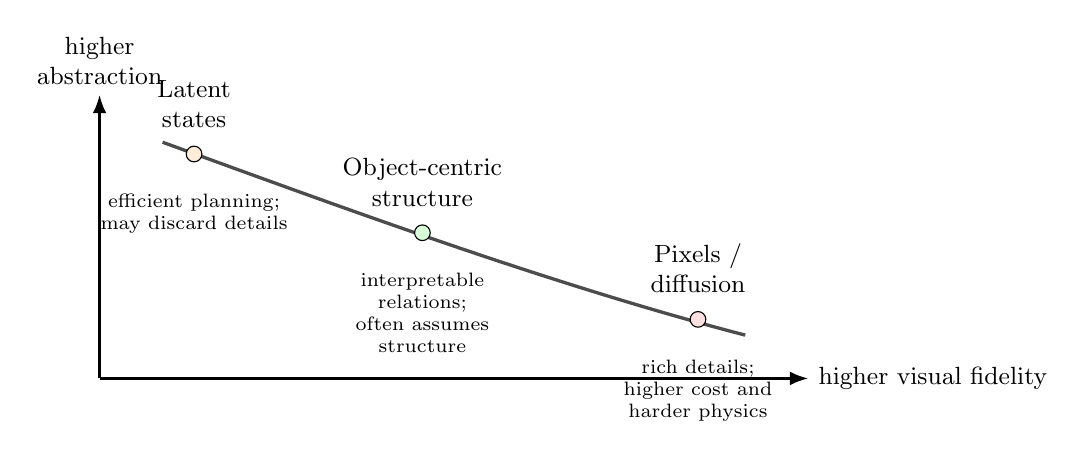
\begin{tikzpicture}[
  point/.style={circle, draw, fill=white, inner sep=2pt},
  label/.style={align=center, font=\small},
  note/.style={align=center, font=\scriptsize, text width=2.7cm}
]
  \draw[thick, -Latex] (0,0) -- (9,0) node[right, font=\small] {higher visual fidelity};
  \draw[thick, -Latex] (0,0) -- (0,3.6) node[above, align=center, font=\small] {higher\\abstraction};
  \draw[very thick, color=black!70] (0.8,3.0) .. controls (3.0,2.2) and (5.7,1.2) .. (8.2,0.55);
  \node[point, fill=orange!15] (latent) at (1.2,2.85) {};
  \node[label, above=3pt of latent] {Latent\\states};
  \node[note, below=8pt of latent] {efficient planning;\\may discard details};
  \node[point, fill=green!15] (object) at (4.1,1.85) {};
  \node[label, above=3pt of object] {Object-centric\\structure};
  \node[note, below=8pt of object] {interpretable relations;\\often assumes structure};
  \node[point, fill=red!12] (diff) at (7.6,0.75) {};
  \node[label, above=3pt of diff] {Pixels /\\diffusion};
  \node[note, below=8pt of diff] {rich details;\\higher cost and harder physics};
\end{tikzpicture}
\caption{The abstraction-fidelity trade-off. Latent models emphasize compact state for planning, object-centric models add interpretable structure, and pixel or diffusion models preserve visual detail but require stronger evaluation for rollout validity and physical consistency.}
\label{fig:abstraction_fidelity}
\end{figure}

\subsection{From Video Rollouts to Compact Latent Simulators}

The early recurrent world-model formulation crystallized the idea that a learned latent model can act as a simulator for downstream control. The model factorizes perception, memory, and action into a VAE, an MDN-RNN, and a controller, compressing observations into latent vectors and predicting future latent dynamics rather than rolling pixels forward directly \cite{ha2018_world_models_prov}. In this view, the world model is not merely a video predictor with a smaller output space. It is a representation of the environment that can be queried by a policy, optimized inside, or used as a surrogate environment for behavior search.

This modular formulation also exposes a recurring tension in latent world modeling. Policies can be trained inside a hallucinated environment and transferred back to the real one, but this makes simulator fidelity a central concern \cite{ha2018_world_models_prov}. If the learned dynamics are inaccurate in control-relevant regions, the controller may exploit model errors or fail when transferred. This concern is best treated as a limitation and open question rather than as a fully characterized failure mode. The section therefore treats latent simulators as powerful control substrates whose reliability must be judged by how they are used, not only by how well they reconstruct observations.

Token-based interactive world models extend this latent-simulator idea by replacing continuous recurrent states with discrete visual or interaction tokens. iVideoGPT is included in this survey as a recent bridge between VideoGPT-style tokenized video generation and interactive world modeling \cite{wu2024ivideogpt}. Its role here is to mark a design direction in which autoregressive token dynamics become part of the world-model family, not to suggest that token models supersede the recurrent VAE/RNN or RSSM lineage.

\subsection{RSSM Dynamics and Online Planning}

PlaNet made the latent-control formulation more systematic by planning directly in a recurrent state-space model. Its RSSM combines deterministic memory with stochastic latent variables, learns observation and reward models, and performs online model-predictive control by searching candidate action sequences in latent space \cite{hafner2019_planet_prov}. Figure~\ref{fig:planet-rssm} illustrates the RSSM design used for compact latent planning. This design separates the role of image generation from the role of decision making: decoded images may be useful for training or diagnostics, but planning itself uses latent states and predicted rewards. In the taxonomy of this survey, PlaNet therefore marks a clear move from image-space prediction toward compact state dynamics for action selection.

\begin{figure}[t]
    \centering
    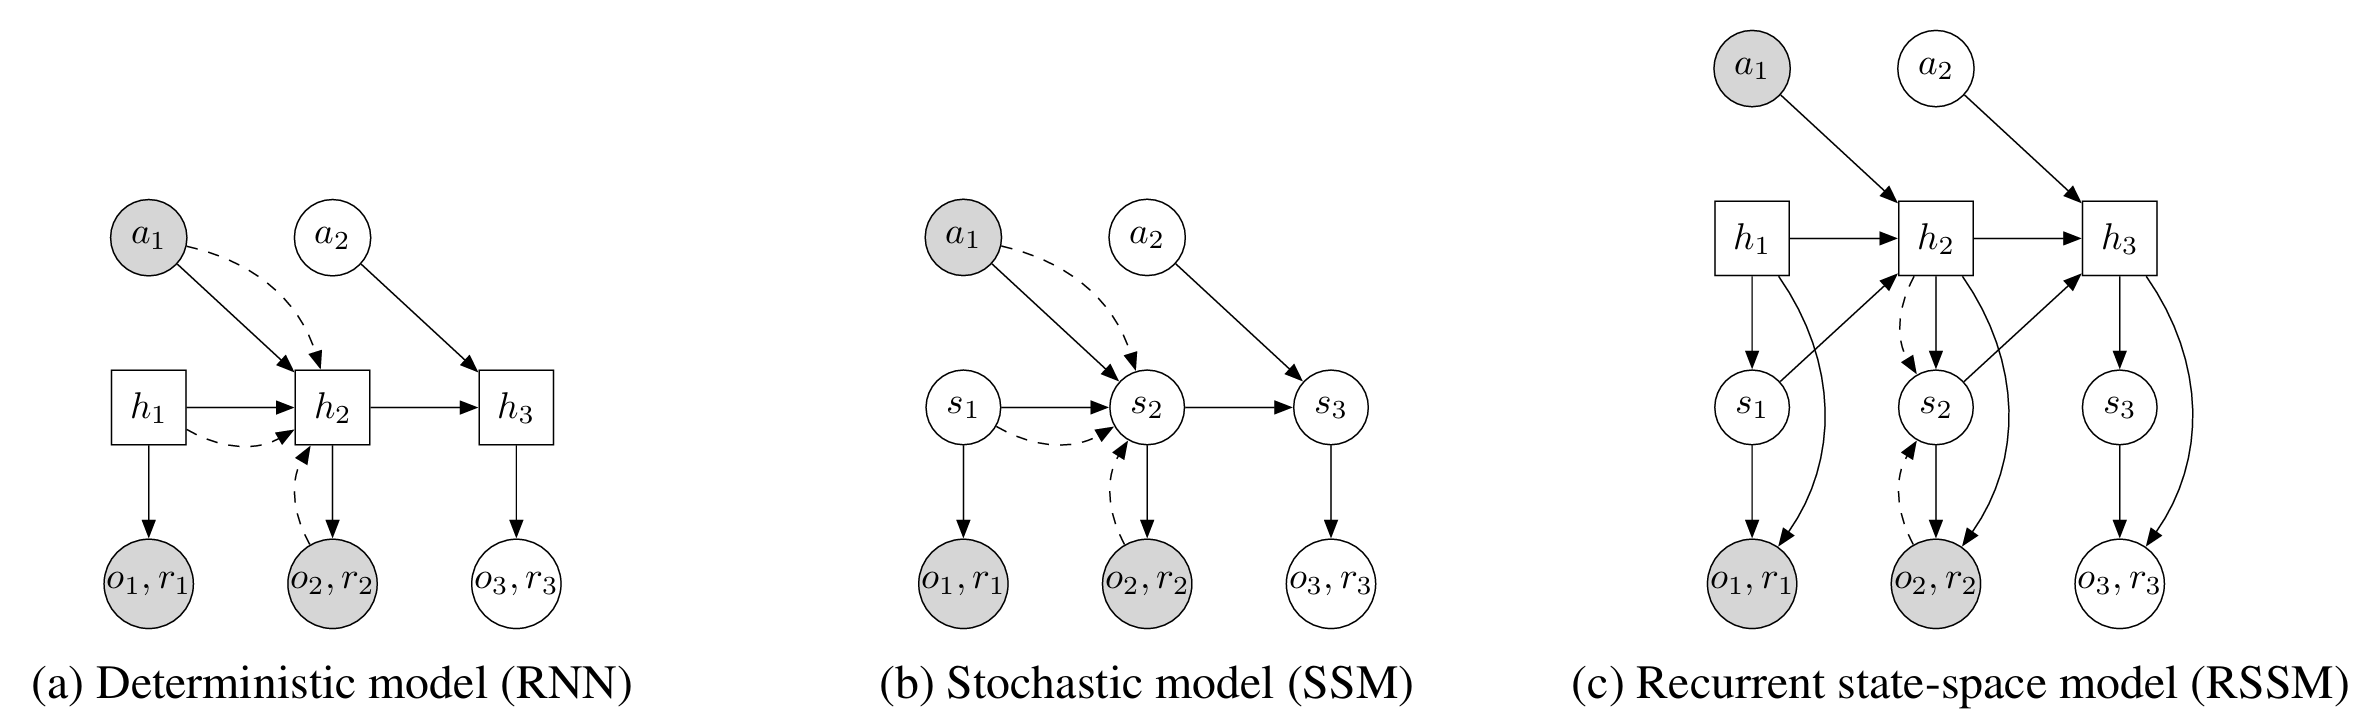
\includegraphics[width=0.88\linewidth]{../figures/planet_rssm.png}
    \caption{Recurrent state-space modeling for latent planning. PlaNet compares deterministic recurrent dynamics, stochastic state-space dynamics, and a recurrent state-space model that combines deterministic memory with stochastic latent variables. The RSSM design enables planning over compact latent states rather than over full image rollouts. Reproduced/adapted from Hafner et al.~\cite{hafner2019_planet_prov}.}
    \label{fig:planet-rssm}
\end{figure}

RSSM-style models also illustrate why the internal structure of the latent state matters. PlaNet's deterministic and stochastic components are important for performance, suggesting that latent world models need both memory for partial observability and uncertainty-aware state variables for prediction \cite{hafner2019_planet_prov}. This is not the same as the stochastic video-prediction problem in Section~\ref{sec:video_prediction}: here, uncertainty is embedded in a control-oriented state that is trained with observation and reward objectives. The relevant question becomes whether the latent state preserves the information needed for planning, not whether every generated frame is visually sharp.

Feature-space predictive models offer a different contrast to RSSM-style generative latent states. V-JEPA 2 is a self-supervised video model for understanding, prediction, and planning, with a latent representation rather than an explicit pixel decoder at the center of the discussion \cite{assran2025vjepa2_prov}. This makes it useful for comparing generative latent prediction with non-generative feature prediction. The cautious methodological claim is that feature-space predictors raise the question of whether planning-relevant state can be learned without reconstructing observations at every step.

\subsection{Latent Imagination and Policy Learning}

Dreamer changes the role of the latent model from an online planner to an imagination engine for policy learning. Instead of searching over action sequences at each decision point, Dreamer trains an actor and critic from imagined latent trajectories, using gradients through the learned dynamics and value estimates \cite{hafner2020_dreamer_prov}. This amortizes decision making into a learned policy and makes the world model a training substrate for long-horizon behavior. The conceptual shift is important: the learned dynamics are no longer only a model to plan through at test time, but a generator of imagined experience for updating behavior.

This imagination-based formulation strengthens the case that world-model evaluation differs from visual reconstruction quality. Dreamer is evaluated through visual-control performance and data efficiency, emphasizing behavior learning through latent imagination rather than pixel-space rollout fidelity \cite{hafner2020_dreamer_prov}. Together with PlaNet and the recurrent world-model formulation, this supports the survey's core latent-model claim: compact predictive states can make video-based world modeling useful for planning or policy learning \cite{ha2018_world_models_prov,hafner2019_planet_prov,hafner2020_dreamer_prov}. However, return-based evaluation still does not guarantee physical faithfulness or open-ended simulation quality. A latent model can be useful for a reward-defined task while remaining weak as a general physical simulator.

\subsection{Discrete, Token, Robotic, and Feature-Space Extensions}

Several important modern extensions belong in this conceptual family, including discrete latent world models, transformer or token-based world models, physical robot world models, feature-space planning with pretrained visual representations, and contextualized world-model pretraining from in-the-wild videos. DreamerV2, IRIS, DayDreamer, DINO-WM, ContextWM, iVideoGPT, and V-JEPA 2 are all relevant to this wider design space \cite{hafner2021_dreamerv2_prov,micheli2023_iris_prov,wu2022_daydreamer_prov,zhou2025_dino_wm_prov,wu2023_contextwm_prov,wu2024ivideogpt,assran2025vjepa2_prov}. This section uses them to clarify comparison axes for latent world models rather than to make a detailed cross-paper ranking.

The comparison axes are clear. First, discrete tokens and continuous latent states make different commitments about compression, rollout, and error accumulation. Second, generative latent prediction and non-generative feature prediction differ in whether the model must reconstruct observations or only preserve predictive state. Third, small-domain world models and large-scale video-pretrained models differ in the data regime from which their dynamics are learned. These axes make iVideoGPT and V-JEPA 2 useful additions to the survey's map, but not replacements for PlaNet and Dreamer as the foundational lineage. They should be compared carefully before being folded into stronger claims about the field as a whole.

\subsection{Limits and Transition to Image-Space World Models}

Latent world models trade visual detail for compactness and control utility. This is often a strength: planning in latent space can avoid expensive image rollouts, and actor-critic imagination can reuse a learned model to generate many behavior-learning trajectories \cite{hafner2019_planet_prov,hafner2020_dreamer_prov}. But the same abstraction creates limitations. Latent states are optimized around reconstruction, reward, value, or control objectives, so they may discard details that later matter for action. They are also typically evaluated in specific environments with defined rewards, leaving open questions about physical abstraction, compounding model error, simulator exploitation, and transfer to more complex real-world video.

The abstraction-fidelity trade-off motivates the next section on image-space and diffusion-based world models. PlaNet and Dreamer show why compact latent dynamics are attractive for planning and policy learning; DIAMOND, by contrast, argues that preserving image-space visual details can improve downstream reinforcement learning in Atari \cite{hafner2019_planet_prov,hafner2020_dreamer_prov,alonso2024_diamond_prov}. The transition is therefore not a simple progression from worse to better representations. It is a shift in design pressure: latent models emphasize efficient predictive state for control, while diffusion and interactive models revisit whether richer image-space generation or controllable video synthesis can preserve information that compact latents may lose.

The latent-model family has also diversified internally. Continuous RSSM states, discrete token models, and feature-space predictors occupy different points in the design space, and each raises different evaluation questions about planning utility, physical abstraction, and transfer. The survey therefore treats modern token and feature-space models as complementary pressure tests for the latent-world-model framework, while keeping the core evidence grounded in the recurrent world-model, PlaNet, and Dreamer lineages \cite{ha2018_world_models_prov,hafner2019_planet_prov,hafner2020_dreamer_prov,wu2024ivideogpt,assran2025vjepa2_prov}.

\section{Diffusion-Based and Interactive World Models}

\paragraph{Section thesis.}
Diffusion-based world models revisit image-space simulation with stronger generative machinery, while interactive world models extend prediction from watching video to controlling video worlds.

\paragraph{Planned subsections.}
\begin{itemize}
  \item Image-space diffusion as environment dynamics.
  \item Fidelity versus abstraction in control.
  \item Known actions, robot commands, and latent actions.
  \item Interactive generative environments from unlabeled video.
  \item Physical-correctness limits for visually strong generators.
\end{itemize}

\paragraph{Key claims.}
\begin{itemize}
  \item C015: Conditional diffusion can model image-space environment dynamics. Supporting papers: P012 \cite{alonso2024_diamond_prov}.
  \item C016: Preserving visual details can improve RL performance. Supporting papers: P012 \cite{alonso2024_diamond_prov}.
  \item C017: Diffusion fidelity does not yet establish physical correctness in embodied domains. Supporting papers: P012 \cite{alonso2024_diamond_prov}.
  \item C018: Interactive generative environments can learn latent actions from unlabeled video. Supporting papers: P013 \cite{bruce2024_genie_prov}.
  \item C019: Prediction becomes embodied when futures depend on actions, policies, or latent controls. Supporting papers: P004 \cite{oh2015_action_conditional_video_prediction_prov}, P005 \cite{finn2016_physical_interaction_video_prediction_prov}, P013 \cite{bruce2024_genie_prov}.
  \item C020: Learned latent actions can support downstream imitation in narrow settings. Supporting papers: P013 \cite{bruce2024_genie_prov}.
  \item C021: Visual realism should not be equated with physical correctness. Supporting papers: P037 \cite{bansal2025_videophy_prov}, P012 \cite{alonso2024_diamond_prov}.
  \item C026: Compact latent abstraction and image-space detail preservation create a trade-off. Supporting papers: P001 \cite{hafner2019_planet_prov}, P002 \cite{hafner2020_dreamer_prov}, P012 \cite{alonso2024_diamond_prov}.
\end{itemize}

\paragraph{Expected figures and tables.}
\begin{itemize}
  \item Figure 6: Latent rollout versus image-space diffusion rollout.
  \item Figure 7: Known-action control versus latent-action control.
  \item Table 7: Fidelity, compute, controllability, and evaluation trade-offs.
\end{itemize}

\paragraph{Missing evidence.}
\begin{itemize}
  \item Notes for P011, P020, and P022 are needed before presenting the diffusion lineage. \textbf{[NEEDS SOURCE]}
  \item Notes for P016, P021, P022, and P024 are needed before broad embodied and interactive coverage. \textbf{[NEEDS SOURCE]}
  \item Physical-law evaluation of diffusion rollouts remains under-supported by completed notes. \textbf{[NEEDS SOURCE]}
\end{itemize}

\section{Evaluation and Open Challenges}

\paragraph{Section thesis.}
Evaluating video world models requires combining visual fidelity, control utility, physical commonsense, causal validity, controllability, and long-horizon behavior.

\paragraph{Planned subsections.}
\begin{itemize}
  \item Why visual fidelity is not enough.
  \item Control utility and planning success.
  \item Physical commonsense and material-interaction benchmarks.
  \item Automatic evaluators and human verification.
  \item Open challenges: evaluation, structure, controllability, and abstraction-fidelity.
\end{itemize}

\paragraph{Key claims.}
\begin{itemize}
  \item C003: Frame quality alone is insufficient for world-model evaluation. Supporting papers: P004 \cite{oh2015_action_conditional_video_prediction_prov}, P009 \cite{janner2019_o2p2_prov}, P012 \cite{alonso2024_diamond_prov}.
  \item C021: Visual realism should not be equated with physical correctness. Supporting papers: P037 \cite{bansal2025_videophy_prov}, P012 \cite{alonso2024_diamond_prov}.
  \item C022: Physical-consistency benchmarks can categorize material interactions. Supporting papers: P037 \cite{bansal2025_videophy_prov}.
  \item C023: Automatic evaluators can scale physical-consistency evaluation but still approximate human judgment. Supporting papers: P037 \cite{bansal2025_videophy_prov}.
  \item C024: Evaluation should go beyond pixel fidelity and reward. Supporting papers: P004 \cite{oh2015_action_conditional_video_prediction_prov}, P012 \cite{alonso2024_diamond_prov}, P013 \cite{bruce2024_genie_prov}, P037 \cite{bansal2025_videophy_prov}.
  \item C025: Learning object structure, hidden variables, and interaction dynamics without direct supervision is an open challenge. Supporting papers: P005 \cite{finn2016_physical_interaction_video_prediction_prov}, P007 \cite{battaglia2016_interaction_networks_prov}, P008 \cite{watters2017_visual_interaction_networks_prov}, P009 \cite{janner2019_o2p2_prov}, P013 \cite{bruce2024_genie_prov}.
  \item C026: Compact latent abstraction and image-space detail preservation create a trade-off. Supporting papers: P001 \cite{hafner2019_planet_prov}, P002 \cite{hafner2020_dreamer_prov}, P012 \cite{alonso2024_diamond_prov}.
\end{itemize}

\paragraph{Expected figures and tables.}
\begin{itemize}
  \item Figure 8: Evaluation matrix crossing fidelity, control, physical consistency, and generalization.
  \item Table 8: Evaluation protocols and what they test.
  \item Table 9: Open challenges mapped to evidence gaps.
\end{itemize}

\paragraph{Missing evidence.}
\begin{itemize}
  \item Notes for P033--P036 and P038--P040 are needed before the benchmark discussion is complete. \textbf{[NEEDS SOURCE]}
  \item Direct comparisons among FVD, physical-reasoning benchmarks, prompt-based commonsense benchmarks, and control returns are pending. \textbf{[NEEDS SOURCE]}
\end{itemize}

\section{Conclusion}

\paragraph{Section thesis.}
The conclusion should synthesize the survey's conceptual arc and evidence gaps without introducing new claims.

\paragraph{Planned subsections.}
\begin{itemize}
  \item Recap of the concept-driven taxonomy.
  \item Recap of supported claims.
  \item Evidence gaps that must remain explicit.
  \item Final outlook after remaining notes are completed.
\end{itemize}

\paragraph{Key claims.}
\begin{itemize}
  \item Reuse only claims already established in Sections 3--8.
  \item Do not introduce new technical claims in this section.
\end{itemize}

\paragraph{Supporting papers and citation keys.}
\begin{itemize}
  \item No new citations should be introduced here unless they already appeared in earlier sections.
\end{itemize}

\paragraph{Expected figures and tables.}
\begin{itemize}
  \item Optional final roadmap figure if Figure 1 is not overloaded.
\end{itemize}

\paragraph{Missing evidence.}
\begin{itemize}
  \item Summarize unresolved \textbf{[NEEDS SOURCE]} items from prior sections rather than hiding them.
\end{itemize}


\bibliographystyle{plain}
\bibliography{../bib/references}

\end{document}
